\chapter{Data \& Methods}
\label{metodos}

\section{Methodological Steps}

The primary objective of this thesis was to identify the key dynamical mechanisms influencing cyclone development in the Southwestern Atlantic and Southeast American regions across their various development phases. This was achieved through a series of methodological steps as detailed below and illustrated in Figure \ref{fig:flow_chart}.

A comprehensive database of cyclonic system tracks was used, encompassing all systems with genesis in the South Atlantic region from 1979 to 2020. The cyclones were detected based on their central relative vorticity at 850 hPa using the TRACK algorithm. This extensive dataset served as the foundational input for subsequent analyses.

The CycloPhaser program was developed to delineate the distinct life phases of each cyclone. CycloPhaser decomposes the relative vorticity time series into distinct phases using its maximum, minimum, and derivative values. This tool facilitated the construction of a climatology of cyclone life cycle phases, enabling a detailed investigation of the mean characteristics and spatial distribution of cyclones during each phase of their development.

An application was programmed to compute the Lorenz Energy Cycle (LEC) for all cyclones in the database. This analysis provided insights into the energetics of the systems, allowing for a detailed examination of the mean energy characteristics across different life cycle phases.

To further refine the analysis, the K-means clustering algorithm was employed to identify distinct energy patterns (EPs) within the cyclones. This classification enabled the grouping of cyclones based on their energy characteristics, facilitating a more detailed understanding of the dynamical processes at play.

The final step involved a detailed investigation of the dynamical mechanisms associated with cyclonic system development. By examining absolute vorticity ($\eta$) fields, the Rayleigh-Kuo criterion was employed for detecting the occurrence of barotropic instability during cyclone development, while the occurrence of baroclinic instability was assessed using maximum Eady Growth Rate fields.

\begin{figure}[h!]
  \centering
  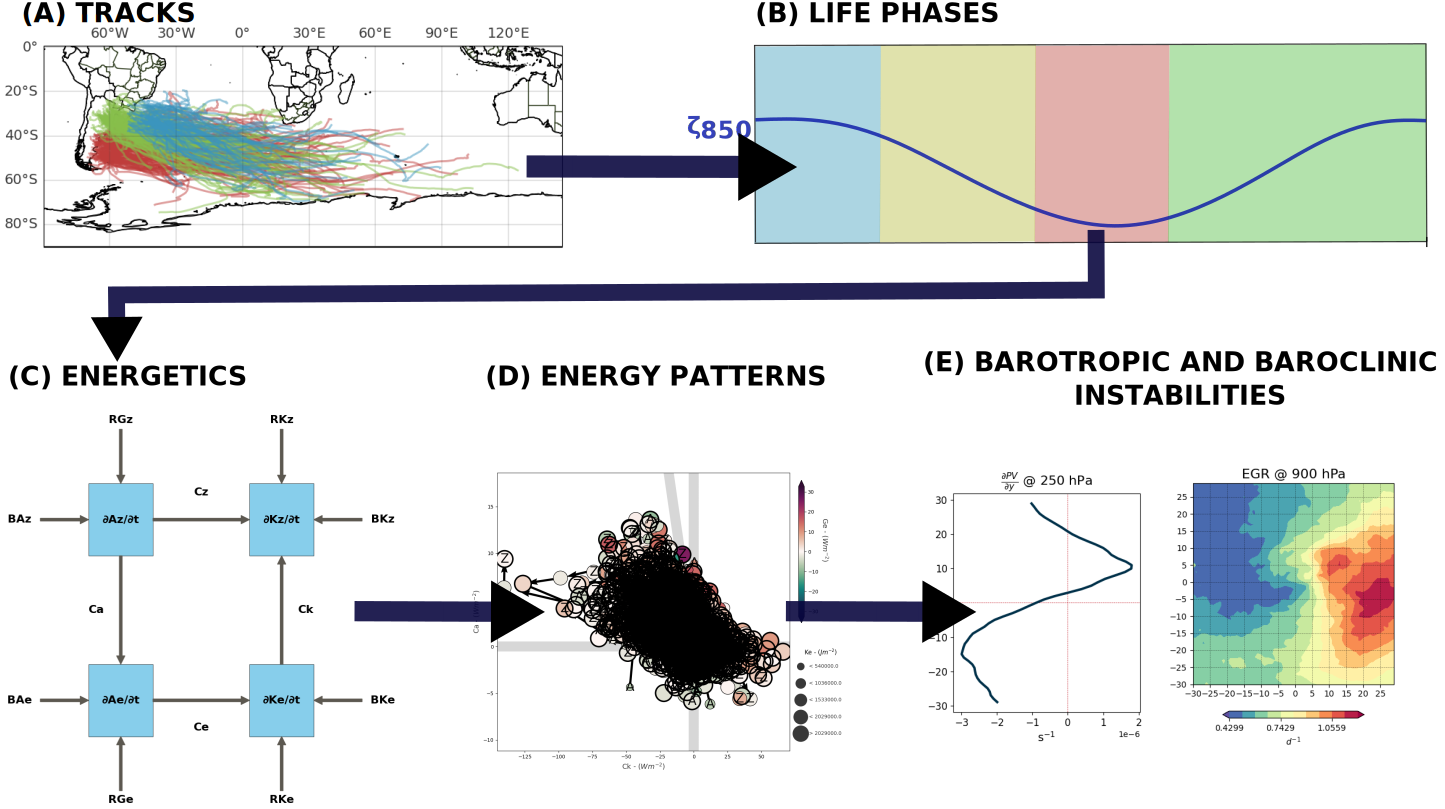
\includegraphics[width=\textwidth]{figs_3/flow_chart.pdf}
  \caption{Flowchart depicting the methodological steps used in this thesis. (A) Retrieval of the cyclonic system track database using central relative vorticity at 850 hPa. (B) Identification of cyclone life phases with CycloPhaser, categorizing the vorticity time series into distinct phases. (C) Computation and analysis of the Lorenz Energy Cycle for the cyclones to investigate their energetic characteristics. (D) Classification of energy patterns using the K-means algorithm to determine distinct energy characteristics. (E) Examination of dynamical mechanisms related to barotropic and baroclinic instabilities influencing cyclone development.}
  \label{fig:flow_chart}
\end{figure}

\section{Databases}

\subsection{ERA5 Reanalysis}
\label{sec:era5}

For both the cyclone tracking procedure and for the energetics computation, the database used was the ERA5 \citep{hersbach2020era5}. The ERA5 is a comprehensive reanalysis dataset developed by the European Centre for Medium-Range Weather Forecasts (ECMWF). It represents the fifth generation of ECMWF reanalysis, providing global climate and weather data with an unprecedented level of detail and accuracy. This dataset spans from January 1940 to the present, with ongoing updates ensuring its relevance for current and historical climate studies.

ERA5 reanalysis data are produced using the Integrated Forecasting System (IFS) Cy41r2, which assimilates a vast array of observations, including satellite and in-situ measurements \citep{hersbach2020era5}. The dataset offers hourly estimates of a multitude of atmospheric, ocean-wave, and land-surface parameters, making it highly valuable for various meteorological and climate research applications. The spatial resolution of ERA5 is approximately 31 km, with 137 vertical levels from the surface to 1 hPa, providing detailed information into the vertical structure of the atmosphere.

The ERA5 reanalysis dataset has been evaluated for the Southern Hemisphere. It can provide precipitation patterns comparable to observations, although the reanalysis presents more accurate results for the extratropics, especially in winter, than for tropical regions \citep{balmaceda2021evaluation,lavers2022evaluation}. The dataset also provides accurate results for surface winds, particularly outside the tropical region, although the associated errors increase with wind intensity \citep{campos2022assessment}. However, for near-surface winds, \citet{ramon2019global} demonstrated that the ERA5 is currently the reanalysis that presents the best results. For temperature, although the ERA5 captures accurately the spatial distribution of temperature indices it can present warm biases near the Andes and on southern South America \citep{balmaceda2021evaluation}. For temperature, while ERA5 accurately captures the spatial distribution of temperature indices, it can present warm biases near the Andes and in southern South America \citep{balmaceda2021evaluation}.


\subsection{Cyclone Tracks in the South Atlantic}
\label{track_method}

For this study, precise information about the positioning (track) and central vorticity at the 850 hPa level (\(\zeta_{850}\)) of cyclones was essential. These data were sourced from the "Atlantic Extratropical Cyclone Tracks Database" as detailed by \citet{gramcianinov2020data}. Spanning from 1979 to 2020, this database covers the entire Atlantic Ocean within the spatial domain of 15\(^\circ\)S–55\(^\circ\)S and 75\(^\circ\)W–20\(^\circ\)E. Cyclone tracking within this database utilizes the ERA5 reanalysis fields, employing the TRACK algorithm \citep{hodges1994general, hodges1995feature} and the method outlined by \citet{hoskins2002new}, which computes relative vorticity from wind components at the 850 hPa level. The TRACK algorithm has previously been used for obtaining cyclone climatologies in the South Atlantic region \citep{gramcianinov2019properties,gramcianinov2020analysis}. The ERA5 dataset was chosen for its superior resolution, offering significant advantages in analyzing regions with complex orography and temperature gradients, such as the SESA region, ensuring a comprehensive and consistent representation of cyclone climatology \citep{gramcianinov2020analysis}.

The tracking criteria included a minimum cyclone duration of 24 hours and a displacement threshold of 1000 km. These requirements align with previous climatologies of South Atlantic cyclones \citep{sinclair1995climatology, gramcianinov2019properties}. Additionally, systems that spent over 80\% of their lifecycle over continental regions were excluded to avoid counting thermal lows and lee troughs, which are not the focus of this study \citep{crespo2021potential}. While the primary focus was on extratropical cyclones, due to the specific calibration and sensitivity of the TRACK algorithm to features typical of these systems, the methodology does not explicitly exclude subtropical or tropical cyclones. Despite their rarity in the South Atlantic, subtropical systems, which occasionally exhibit characteristics similar to extratropical cyclones \citep{hart2003cyclone}, may still be detected but remain a minority in the dataset. Further details on the methodology and database evaluation are discussed in \cite{gramcianinov2020analysis}.


\section{Cyclone's Life Cycle Detection}
\label{sec:cyclone_life_cycle_detection}

This section outlines the procedure for detecting the life cycle phases of cyclones. In the current study, an automated method, the Cyclophaser program, was developed and employed to facilitate this process. Section \ref{sec:cyclophaser_description} provides an in-depth examination of the Cyclophaser program, highlighting its functionalities and the methodologies it employs. Subsequently, Section \ref{sec:cyclophaser_settings} explores the specific settings and configurations of the Cyclophaser used in this study.

\subsection{Cyclophaser Program Description} \label{sec:cyclophaser_description}

To facilitate the detection of individual life cycle phases of cyclones, an automated Python package named Cyclophaser (Figure \ref{fig:cyclophaser_logo}) was developed \citep{deSouza2024}. This package is open-source and freely available on the PyPI repository. It can be installed using the pip package manager with the command \texttt{pip install cyclophaser}. Comprehensive documentation, including usage examples, is available on ReadTheDocs at \url{https://cyclophaser.readthedocs.io/en/latest/}, and the complete source code, which is open to contributions, can be found on GitHub at \url{https://github.com/daniloceano/CycloPhaser}.

\begin{figure}[h]
\centering
\includegraphics[width=\linewidth]{figs_3/cyclophaser.png}
\caption[Cyclophaser - Logo]{The logo of the Cyclophaser program.}
\label{fig:cyclophaser_logo}
\end{figure}

The program is designed to detect cyclone lifecycle phases using series of relative vorticity at the system's central position and its first derivative (Figure \ref{fig:/cyclophaser_methodology}). While Cyclophaser was specifically developed and tested for this purpose, other variables such as sea level pressure or geopotential data might also be effective, although tests using these variables have not yet been conducted. Exploring how the lifecycle of cyclones might vary with different variables and how the geographical positioning of each stage might differ is an open research question.

\begin{figure}[h]
\centering
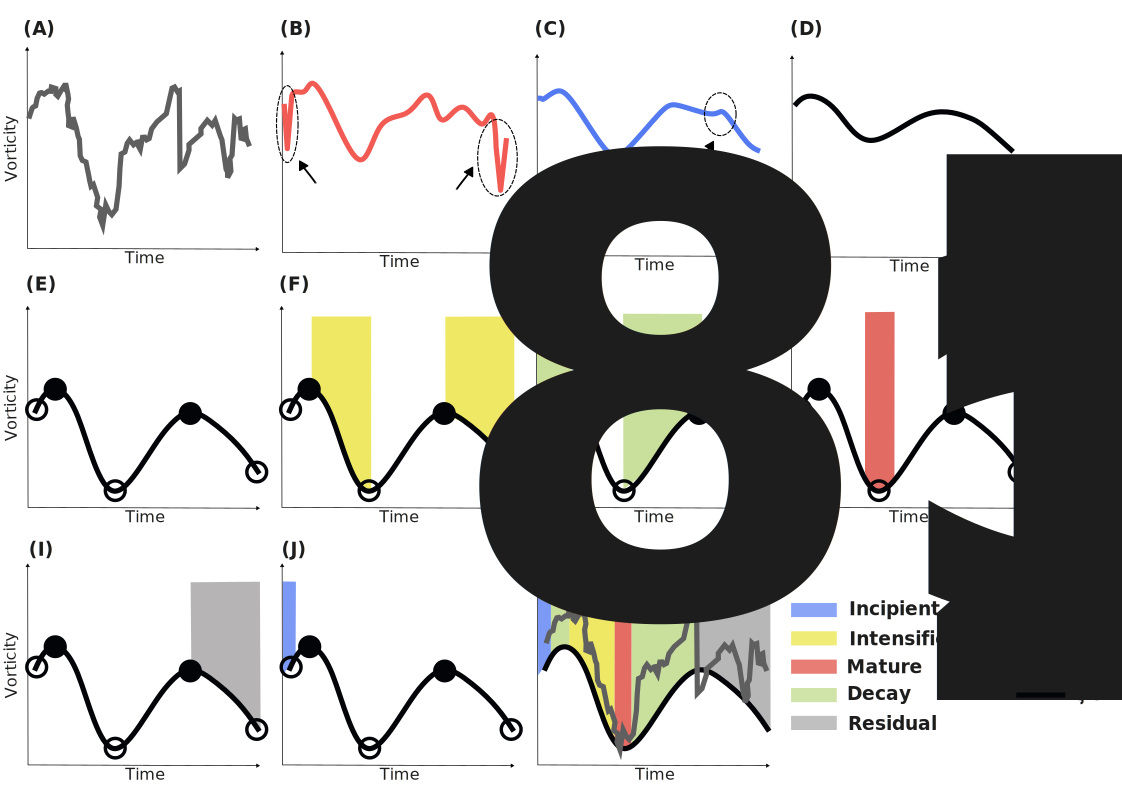
\includegraphics[width=\linewidth]{figs_3/cyclophaser_methodology.pdf}
\caption[Cyclophaser - Methodological Steps]{Illustrative representation of the methodological steps employed by Cyclophaser in analyzing cyclone lifecycle phases using vorticity series. The detailed steps demonstrate the application of data processing techniques including the Lanczos filter.}
\label{fig:/cyclophaser_methodology}
\end{figure}

The program begins with a preprocessing stage where users have the option to apply the Lanczos filter \citep{duchon1979lanczos} to the vorticity time series (Figure \ref{fig:/cyclophaser_methodology}b). Based on the $sinc$ function, the ideal mathematical representation of a low-pass filter, the Lanczos filter is adapted by windowing the $sinc$ function to a finite range. Cyclophaser utilizes a band-pass filtering technique where weights are calculated using two cutoff frequencies, creating a differential of two $sinc$ functions. This allows the filter to pass a specific frequency range while attenuating frequencies outside this range, permitting customization based on the spatio-temporal resolutions of different reanalysis datasets.

The Lanczos filter's primary use in Cyclophaser is to remove noise unrelated to the development of extratropical cyclones on synoptic scales, including fluctuations due to topography-induced circulations, sea breezes, and spatial and temporal variations in sea surface structures \citep{steele2015modelling, da2017shallow, acevedo2010atmospheric}. High-resolution datasets like ERA5 benefit from this filtering, which effectively reduces noise from structures like frontal systems \citep{hoskins2002new}. However, this filtering step may be omitted for datasets that have been preprocessed by tracking algorithms incorporating spatial filters \citep[e.g.]{murray1991numerical, pinto2005sensitivities, flaounas2014cyclotrack, hoskins2002new}.  As the track database used in the present study employed a filtering technique, the Lanczos filtering was not needed. Thus, a detailed formulation, explanation, and exploration of the issues related to such a filtering technique are provided in Appendix \ref{ap01}.

After the initial filtering, the CycloPhaser program employs the Savitzky-Golay filter \citep{savitzky1964smoothing}, as implemented in SciPy's package \citep{virtanen2020scipy}, to further reduce residual noise. This step is crucial for ensuring that the derivative curves form a sinusoidal pattern, which is essential for precise phase detection (Figure \ref{fig:/cyclophaser_methodology}c). The Savitzky-Golay filter operates by fitting a polynomial of degree \( k \) to a window of \( 2m+1 \) data points centered at each point \( y_i \) in the input signal. The coefficients of this polynomial are determined by minimizing the least squares error between the polynomial and the data points within the window. The smoothed value \( \hat{y_i} \) at the point \( y_i \) is then calculated by evaluating the fitted polynomial at \( x_i \):
\[
\hat{y_i} = \sum_{j=-m}^{m} c_j y_{i+j}
\]
where \( c_j \) are the coefficients derived from the polynomial fit, and \( m \) represents half the window size.

Users have the option to apply this smoothing twice (Figure \ref{fig:/cyclophaser_methodology}d), adjusting the window size \( 2m+1 \) and the polynomial order \( k \) to optimize the balance between noise reduction and data fidelity. This flexibility allows users to fine-tune the filter settings to meet specific requirements based on the spatio-temporal resolutions of various reanalysis datasets.

Subsequently, the first derivative of the relative vorticity is calculated predominantly using second-order finite differences, with central differences applied to interior points and first-order forward or backward differences used for endpoints. This derivative is then subjected to double smoothing with the Savitzky-Golay filter to maintain a sinusoidal pattern in the derivative series. This step is critical for accurately identifying cyclone lifecycle phases, making the dual smoothing process mandatory; omitting this could result in a noisy derivative series, potentially leading to erroneous phase detections, which emphasizes its necessity for reliable analysis.

The first phases to be detected are the intensification and decay stages. The program achieves this by analyzing peaks and valleys in the relative vorticity time series data, as shown in Figure \ref{fig:/cyclophaser_methodology}e. The intensification phase is defined as the period between a peak and the subsequent valley (Figure \ref{fig:/cyclophaser_methodology}f). Conversely, the decay phase is defined as the interval between a valley and the following peak (Figure \ref{fig:/cyclophaser_methodology}g). To ensure that only significant phases are considered, each intensification and decay interval must span at least 7.5\% of the total length of the time series. This threshold helps filter out minor fluctuations that are not indicative of true phase changes. To further refine the accuracy of phase detection, the program checks for multiple blocks of consecutive intensification or decay periods. If the gap between these blocks is smaller than 7.5\% of the total series length, the program merges them into a single period. This merging process is crucial as it prevents the fragmentation of significant phases due to short gaps, thereby providing a more accurate and continuous representation of the intensification and decay stages.

After detecting the intensification and decay stages, the program proceeds to identify the mature stage of the cyclone's life cycle (Figure\ref{fig:/cyclophaser_methodology}h). This stage is determined by analyzing not only the peaks and valleys in the relative vorticity but also the smoothed derivative of vorticity. Between a peak and the subsequent valley (or a valley and the subsequent peak) of the vorticity series, there is always a corresponding valley (or peak) in its derivative. These points indicate periods of maximum intensification or decay of vorticity. The mature stage is defined as the interval between a vorticity valley and an adjusted point calculated based on the derivative of vorticity. Specifically, the mature stage spans from 12.5\% of the time between the preceding derivative valley to 12.5\% of the time to the following derivative peak. To be recognized as a significant mature stage, each interval must span at least 3\% of the total length of the time series. This threshold ensures that only substantial periods are classified as mature stages. Additionally, the program verifies that all mature stages are preceded by an intensification stage and followed by a decay stage. This verification step ensures that the mature phase is accurately identified within the context of the entire cyclone life cycle.

Our methodology introduces the 'residual' stage, which is not directly related to the intrinsic development of extratropical cyclones but rather to peculiarities arising from the tracking algorithms (Figure \ref{fig:/cyclophaser_methodology}i). This stage is exemplified in Figure \ref{residual_study_case}. Panel (a) illustrates the intensification of a cyclonic system near the southernmost part of Argentina. The system reaches maturity, characterized by closed isobars at 850 hPa (Panel b). As the system begins to decay, it displays open isobars and diminished relative vorticity cohesion (Panel c). During its decay, it is influenced by a nearby system that leads to a temporary increase in the magnitude of its central relative vorticity, indicating a temporary re-intensification (Panel d). The tracking algorithm eventually discontinues its tracking, categorizing this late period of intensification as 'residual'—a phase of late intensification that is not associated with the primary development of the cyclone, as depicted in the relative vorticity series (Panel e).

\begin{figure}[h!]
\centering
\includegraphics[width=37pc]{figs_3/residual_study_case_edited.pdf}
\caption[Residual Stage - Study case]{Relative vorticity (shaded) and geopotential heights (contours) at 850 hPa, illustrating distinct stages of a cyclone's lifecycle where a residual stage is present. Panel (A) shows the intensification stage with isobars still open, indicating a strengthening system. Panel (B) depicts the mature stage, characterized by maximum organization and extent. Panel (C) illustrates the decay stage, with open isobars and reduced relative vorticity cohesion. Panel (D) captures the residual phase, where, despite a general trend of weakening, there is a temporary increase in vorticity influenced by external factors, not directly associated with the primary development of the cyclone. The complete lifecycle of the system is depicted in Panel (E), where each red dot on the vorticity series corresponds to the specific moments shown in Panels (A) to (D).}
\label{residual_study_case}
\end{figure}

The CycloPhaser classifies stages as residual by analyzing the previously detected cyclone phases. For phases classified as mature that do not transition to a decay stage, these instances are classified as residual. Similarly, if a full cycle of intensification, maturity, and decay is followed by another intensification that does not lead to a mature phase, it is also classified as residual (Figure \ref{fig:/cyclophaser_methodology}i). This criterion accounts for scenarios where the tracking algorithm may continue to follow a cyclone post-decay, potentially capturing a re-intensification that does not culminate in a mature stage due to tracking limitations.

Following the residual phase classification, a post-processing step is applied to refine cyclone phase identification. This step bridges any gaps that may appear between consecutive periods identified as intensification or decay phases. Specifically, the program scans for discontinuities within consecutive phase blocks and fills any identified gaps with the adjacent phase to ensure smooth and continuous phase transitions. Additionally, this step involves correcting isolated phases—those misclassified phases that last only one time step—by aligning them with the subsequent phase if they occur at the start of the series, or with the preceding phase elsewhere. This adjustment enhances the consistency of phase identification throughout the cyclone lifecycle.

Ironically, the final step of the CycloPhaser program involves identifying the incipient stage, which marks the beginning of cyclone development (Figure \ref{fig:/cyclophaser_methodology}j). Initially, all undefined periods in the time series are labeled as incipient. Subsequently, the program analyzes the sequence of already labeled phases. If the life cycle commences with an intensification phase, the program searches for a vorticity valley preceding the next mature stage. Should such a valley be present, it designates the period from the start of the intensification phase to 40\% of the duration to this valley as incipient. Conversely, if the life cycle starts with a decay phase, the program looks for a subsequent vorticity peak before the next mature stage. Upon identifying such a peak, it marks the time from the start of the decay phase to 40\% of the duration to this peak as incipient.

The specific thresholds for phase detection, including the 7.5\% duration for intensification and decay intervals, the 3\% minimum for the mature stage, and the 12.5\% intervals defining the boundaries of the mature stage, along with 40\% of the series length for the incipient stage, were established through rigorous testing. This testing involved an iterative trial-and-error calibration process where various percentage thresholds were applied to a representative sample of cyclone tracks. The objective was to determine the most accurate parameters for delineating the phases. The chosen percentages proved effective in capturing the true progression of cyclogenesis while filtering out inconsequential fluctuations in vorticity. This meticulous calibration ensures that the CycloPhaser program reliably identifies each phase, providing a consistent and objective methodology for analyzing the life cycle of extratropical cyclones. This process is illustrated in Figures \ref{fig:threshold_intensification} and \ref{fig:threshold_decay}, \ref{fig:threshold_mature}, \ref{fig:threshold_incipient}. For most of these thresholds, and in most cases analyzed, even altering the parameters to 25\% or 150\% of their original values did not result in significant modifications to the identified life cycle, reinforcing the method's reliability.


\begin{figure}[h!]
    \centering
    \includegraphics[width=\textwidth]{figs_3/figure_threshold_intensification_length.png}
    \caption[Impact of Varying Threshold Values for Intensification Phase]{Impact of varying threshold values for the minimum length of the intensification phase across the six study cases. The original threshold value is maintained at 7.5\% of the cyclone's total life cycle duration in panel (i). Panels (ii) to (vii) depict variations where the threshold is adjusted from 25\% to 175\% of the original value, illustrating the method's sensitivity to threshold changes. Adapted from \citet{deSouza2024}.}
    \label{fig:threshold_intensification}
\end{figure}

\begin{figure}[h!]
    \centering
    \includegraphics[width=\textwidth]{figs_3/figure_threshold_decay_length.png}
    \caption[Impact of Varying Threshold Values for Decay Phase]{Same as Figure \ref{fig:threshold_intensification}, but for the minimum length of the decay phase. Adapted from \citet{deSouza2024}.}
    \label{fig:threshold_decay}
\end{figure}

\begin{figure}[h!]
    \centering
    \includegraphics[width=\textwidth]{figs_3/figure_threshold_mature_length.png}
    \caption[Variations in Threshold Values for Mature Phase]{Variations in threshold values for the time intervals between the valley of vorticity and the preceding derivative valley, as well as from the vorticity valley to the subsequent derivative peak, used for determining the mature stage. The original threshold is set at 12.5\%. Subsequent panels adjust this threshold from 25\% to 175\% of the baseline value, evaluating the robustness of phase detection across six study cases. Adapted from \citet{deSouza2024}.}
    \label{fig:threshold_mature}
\end{figure}

\begin{figure}[h!]
    \centering
    \includegraphics[width=\textwidth]{figs_3/figure_threshold_incipient_length.png}
    \caption[Impact of Varying Threshold Values for Incipient Phase]{Impact of varying the minimum length threshold for the incipient phase of cyclone development. The incipient phase is identified from the beginning of the vorticity series to the next peak or valley in vorticity. The original threshold (shown in panel i) is set based on a percentage of the total vorticity series length. Panels ii to vii display the results when this threshold is modified from 25\% to 175\% of its original value across six study cases. Adapted from \citet{deSouza2024}.}
    \label{fig:threshold_incipient}
\end{figure}

\subsection{Cyclophaser Settings} \label{sec:cyclophaser_settings}

In this study, the default settings of the CycloPhaser were primarily utilized to identify the life cycle phases of cyclones. Since the TRACK algorithm already incorporates spatial filtering on the \(\zeta_{850}\) vorticity fields, application of the Lanczos filter was deemed unnecessary \citep{hodges1994general, hodges1995feature}. Nevertheless, the Savitzky-Golay filter was applied twice to ensure that the \(\zeta_{850}\) series exhibited a smooth sinusoidal profile. The window length of this filter was adjusted specifically for each system's life cycle duration: for systems with a total life cycle spanning 8 days, the window length was set to an odd integer approximately 25\% of the series length. For systems with shorter life cycles, the window length was adjusted to an odd integer approximately 50\% of the series length. In the second smoothing process, for life cycles exceeding 8 days, the window length was set to an odd integer close to 50\% of the series length; however, for shorter cycles, it was kept consistent with the initial smoothing step.

\section{Lorenz Energetics Computation}\label{sec:lec_computation}

To compute the Lorenz Energy Cycle (LEC), an open-source Python application named "lorenz-cycle" was developed and is available on GitHub. The application is designed for collaboration and transparency, allowing peers to freely use, modify, and review the computation procedures. Full documentation and a user guide with illustrative examples can be found at \url{https://github.com/daniloceano/lorenz-cycle}. The program uses the formulation described at Section \ref{math} and its complete description can be found at Appendix \ref{ap02}.

In this study, the lorenz-cycle program was configured to compute the dissipation terms as residuals, following the methodologies of \citet{brennan1980zonal,michaelides1987limited,veiga2008analysis,pezza2010environmental,dias2011energy}, and to use the Semi-Lagrangian framework \citep{michaelides1999quasi}. A $15^\circ \times 15^\circ$ computational domain centered at the cyclone's central position, obtained from the TRACK database (Section \ref{track_method}), was created for each time step. Given the impracticality of manually selecting an appropriate domain size for each cyclone in the dataset, a fixed size was employed.

The focus here is on the environmental energetics directly related to cyclone development, aiming to minimize interactions with other non-related circulations while capturing the main structure of the cyclone. Defining cyclone size is challenging due to both methodological and physical factors \citep[e.g.]{rudeva2007climatology}. The choice of a $15^\circ \times 15^\circ$ computational domain is justified as it is large enough to capture the effective radius of most cyclonic systems \citep{rudeva2007climatology}. The effective cyclone radius is defined as a measure of cyclone size, determined by establishing a coordinate system centered on the cyclone and measuring the distance at which the radial pressure gradient first falls to zero. This domain size also accounts for the cyclone's structure \citep[e.g.]{gramcianinov2019properties}.

Given the primary interest in the Southwestern Atlantic Ocean, only cyclones with genesis near the South American coast (ARG, LA-PLATA, and SE-BR genesis regions) were included in the LEC computation. A significant challenge in determining energetic patterns across this dataset is the variable life durations of cyclones. Averaging values across the entire life cycle of systems would aggregate distinct dynamical processes (e.g., intensification and decay), while technical limitations exist in dissecting the life cycle into distinct periods. For example, \citet{black2013universal} averaged cyclone energetics over periods of 48 hours before explosive cyclogenesis, during explosive deepening, and for 24 and 72 hours after it. However, cyclone life cycles can range from less than 24 hours to over 10 days \citep{trigo2006climatology,reboita2010south,gramcianinov2019properties}, presenting significant physical limitations to such approaches. To address these limitations, the Cyclophaser program was used. After computing the LEC for each system, Cyclophaser was employed to define the life cycle phases for all analyzed systems, and then the mean LEC values for each phase were computed. The files containing the mean LEC results for each development phase are available on GitHub at \url{https://github.com/daniloceano/energetic_patterns_cyclones_south_atlantic}.

\section{Analysis methods}

\subsection{Probability Density Functions}

In the present study, the probability density functions (PDFs) of distinct variables analyzed were represented using the Kernel Density Estimation (KDE) from the Python open-source library Seaborn \citep{waskom2021seaborn}. KDE is a non-parametric method employed to estimate the PDF of a continuous random variable \citep{parzen1962estimation,rosenblatt1956estimation}. Unlike parametric approaches that assume a specific distribution form, KDE makes minimal assumptions about the underlying data distribution, providing flexibility and robustness in density estimation. The technique involves placing a kernel — a symmetric, smooth function, typically Gaussian — on each data point and summing the contributions from all kernels to produce a smooth, continuous estimate of the PDF. The bandwidth of the kernel, a crucial parameter, controls the level of smoothing: a smaller bandwidth captures more details of the data's structure, while a larger bandwidth yields a smoother, more generalized density function. KDE is particularly useful in visualizing the distribution of data and identifying features such as multimodality, skewness, and the presence of outliers, making it a valuable tool in exploratory data analysis and various scientific applications.


\subsection{Cyclone Track Densities}

The spatial statistics from the TRACK program were produced using the spherical kernel method developed by \citet{hodges1996spherical}. This method provides a robust framework for estimating statistical properties from feature track data on a global scale. Unlike previous exponential kernels, these spherical kernels — such as power, quadratic, and biweight kernels — are computationally efficient and locally defined, meaning their influence is confined to a local region around each data point. The spherical kernel estimation is achieved by calculating probability density functions directly on the sphere, thus avoiding distortions caused by projection methods. This method includes an adaptive smoothing technique that adjusts the smoothing parameter based on local data density, ensuring optimal balance between detail retention and noise suppression. Cross-validation is employed to determine the optimal smoothing parameters, enhancing the reliability of the statistical estimates. This approach is particularly valuable for analyzing climatological data.

\subsection{Statistical Analysis}

To determine if there were significant differences in LEC terms across different phases of cyclone life cycles, we conducted a series of statistical tests. Initially, we assessed the assumptions required for Analysis of Variance (ANOVA), which included normality and homogeneity of variances. Normality was evaluated using the Shapiro-Wilk test, and homogeneity of variances was assessed using Levene's test. All statistical tests performed here were employed using the open source Python package SciPy \citep{2020SciPy-NMeth}.

We used the Shapiro-Wilk test to assess the normality of each term's distribution. The p-value from this test indicates whether the data significantly deviate from a normal distribution. A p-value greater than 0.05 implies that the data do not significantly deviate from normality, indicating that the assumption of normality is met.

Levene's test was used to evaluate the homogeneity of variances across different phases for each term. The test statistic indicates the extent to which variances are equal across groups. A high Levene's test statistic suggests greater differences in variances. The p-value associated with Levene's test statistic indicates the probability that the observed differences in variances could have occurred by chance. A p-value greater than 0.05 suggests that the variances are not significantly different across the phases, implying that the assumption of homogeneity is met.

Given that many of our data sets did not meet these assumptions, we primarily employed the non-parametric Kruskal-Wallis (KW) test, which does not assume normality or equal variances, to compare the distributions of each term across different phases. The KW test is particularly useful when the data do not follow a normal distribution or exhibit heterogeneous variances.

The KW test statistic measures the extent to which the medians of the groups differ. A higher KW statistic value indicates a greater difference between group medians. The corresponding p-value for the KW test statistic indicates the probability that the observed differences in medians could have occurred by chance. A p-value less than 0.05 suggests significant differences among the phases for that term.

To compare the vorticity data among different clusters, we conducted a non-parametric statistical analysis due to the non-normal distribution of the data. Initially, we used the KW test to assess if there were statistically significant differences in the vorticity distributions across the clusters. Following the identification of significant differences with the KW test, we performed pairwise comparisons using the Mann-Whitney U test to determine which specific clusters differed significantly. The Mann-Whitney U test is also non-parametric and assesses whether the distributions of two independent groups are different. For each pairwise comparison, the test yields a U statistic and a p-value, where a p-value less than 0.05 indicates a significant difference between the clusters. All statistical analyses were executed using the SciPy package \citep{2020SciPy-NMeth}, and significant differences were visually annotated on box plots to enhance interpretability.

\subsection{Empirical Orthogonal Functions}

To understand the dominant LEC variability patterns within the TRACK dataset, an Empirical Orthogonal Function (EOF) analysis was employed using the Python open-source library pyEOF \citep{zheng_2021}. EOF analysis is a statistical technique used to identify the dominant modes of variability in spatial-temporal datasets \citep{fukuoka1951study,lorenz1956empirical}. It is one of the most used methods in atmospheric sciences, widely adopted for exploratory analysis \citep{hannachi2007empirical}. The method involves decomposing the dataset into orthogonal patterns by performing an eigenvalue decomposition on the covariance matrix of the data. Each EOF represents a spatial pattern, while the associated time series, or Principal Component (PC), describes the temporal evolution of that pattern. This analysis reduces the dimensionality of the dataset, retaining the most significant variability, and is particularly useful for uncovering underlying structures and patterns in complex environmental data. In this context, instead of representing a spatial pattern, each EOF presents a mode of variability of the LEC, while the PCs represent the evolution across distinct cyclones.

\subsection{K-means Algorithm}

In the present study, the K-mean algorithm was used for determining the energetic patterns associated with the cyclones in the SESA region. The K-Means algorithm \citep{macqueen1967} is an iterative clustering method that partitions a dataset into \( K \) distinct clusters, where each data point belongs to the cluster with the nearest mean (centroid). The choice of \( K \), the number of clusters, is crucial and is based on calculations to obtain ideal values that explain the maximum variability. The initial theory of K-Means was improved by \citet{DavidVassilvitskii2007} with the creation of K-Means++, which is used for initializations in the K-Means implementation of the Python package "Scikit-Learn" \citep{scitkit-learn}, utilized in this study. Instead of choosing all centroids randomly, K-Means++ selects the first centroid randomly and then chooses subsequent centroids based on a probability distribution proportional to the squared distance of data points to the nearest already chosen centroid. This increases the likelihood that the initial centroids are spread out across the data, reducing the probability of convergence to a local optimum. In each iteration, the points are assigned to the cluster whose centroid is closest. After the assignment, the centroids are recalculated as the mean of the points assigned to each cluster. This calculation is performed until convergence, which the user can define as the maximum number of iterations. At the end of these updates, the algorithm returns the final clusters. The algorithm iterates between the steps of cluster assignment and centroid updating until a stopping criterion is met. Typically, the algorithm terminates when the centroids do not move significantly between consecutive iterations or when a maximum number of iterations is reached.

Before applying the K-Means algorithm, we used the Elbow Method, a technique designed to determine the optimal number of clusters. This method seeks a balance between the explained variance and the number of clusters by identifying the inflection point in the decrease of explained variance. Specifically, by plotting the explained variance against the number of clusters, the inflection point on the graph indicates the optimal cluster count \citep{Thorndike1953}.

\section{Investigation of Dynamical Mechanisms}\label{sec:ibc_ibt_analysis}

\subsection{Criteria Used}\label{sec:method_criteria}

In this study, we utilized the Rayleigh–Kuo criterion for barotropic instability to determine the presence of instability within cyclonic systems \citep{rayleigh1895stability,kuo1949dynamic}. According to this criterion, the necessary condition for barotropic instability is the existence of a point where the gradient of absolute vorticity (\(\eta\)) with respect to the meridional direction is zero and changes sign within the flow. This can be mathematically expressed as:

\begin{equation}\label{eq:rayleigh_kuo_criteria}
    \frac{\partial \eta}{\partial y} = 0
\end{equation}

Meanwhile, baroclinic instability was acessed using the Eady growth rate, a quantitative measure of the maximum rate of growth for baroclinic instabilities. This is a measure of the maximum rate at which baroclinic instability can amplify disturbances in a stratified fluid, formulated by \citet{hoskins1990existence} as: 

\begin{equation}\label{eq:eady_geowth}
 \sigma_E = 0.31 \frac{f}{N} \left| \frac{\partial u}{\partial z} \right| 
\end{equation}

where \(f\) is the Coriolis parameter, \(\frac{\partial u}{\partial z}\) represents the vertical wind shear and \(N\) is the Brunt-Väisälä frequency, a measure of the stability of the stratification in a fluid such as the atmosphere or ocean. It is given by the formula:

\begin{equation}
N = \sqrt{\frac{g}{\theta} \frac{d\theta}{dz}}
\end{equation}

where \(g\) is the acceleration due to gravity, \(\theta\) is the potential temperature and \(\frac{d\theta}{dz}\) is the vertical gradient of potential temperature.

A larger value of \(N\) indicates greater stability, meaning the atmosphere is more resistant to vertical displacements. The Eady's growth rate highlights the exponential growth of certain atmospheric disturbances under favorable conditions of wind shear and stability.

\subsection{Composites}

For applying the criteria described in Section \ref{sec:method_criteria}, a composite procedure was implemented. Firstly, it was necessary to determine the vertical levels at which baroclinic and barotropic instabilities are indicated to be occurring, using the vertical profiles of $C_A$ and $C_E$, respectively. Then, mean values for atmospheric fields for the ERA5 reanalysis were computed for the intensification phase at these vertical levels. The atmospheric fields used were zonal, meridional, and vertical wind components, temperature, and geopotential.

For the composites using the Semi-Lagrangian framework, firstly, the mean atmospheric fields for the intensification phase for each system were averaged. These mean atmospheric fields were then re-gridded to a non-dimensional spatial domain. Given that the ERA5 reanalysis has a $0.25^\circ$ horizontal spatial resolution, each mean field contained 60 grid points ($15^{\circ} \times 15^{\circ}$). As the Semi-Lagrangian domains are centered on the cyclone's center, the composite domain ranged from -30 to 30 in both the x and y axes.

Furthermore, the differences between the Semi-Lagrangian and Fixed frameworks were also assessed. While the methodology for the Semi-Lagrangian framework is explained in Section \ref{sec:lec_computation}, a distinct approach had to be taken for the Fixed framework. For each system analyzed, a computational domain was automatically detected by using the minimum and maximum latitude and longitude values, adding a $15^{\circ} \times 15^{\circ}$ buffer. By doing so, it is ensured that the system's complete development cycle is represented in the LEC computation.

For the composite procedure, firstly, the meteorological fields were averaged for each computational domain during the intensification phase. Then, the minimum and maximum latitude and longitude values across all fixed computational domains were detected. After this, a synthetic domain was built using these coordinates, and the mean meteorological fields were interpolated to this domain. Finally, the results interpolated to the common grid for each case were averaged into a single composite.


% \begin{itemize}
%     \item Programa de calculo do LEC (Github) e procedimentos adotados para os cálculos
% \end{itemize}

% \section{Determinação dos padrões energéticos}

% \begin{itemize}
%     \item Padronização da duração dos sistemas através do ciclo de vida
%     \begin{itemize}
%         \item Cyclophaser
%     \end{itemize}
%     \item Diagrama de fase (Lorenz Phase Space)
%     \item Cálculo da PCA dos termos
%     \item Método K-means

% \end{itemize}

% \section{Descrição do MPAS-A}

% \begin{itemize}
%     \item Visão geral do modelo
%     \item  Descrição do núcleo dinâmico e discretizações numéricas
%     \item Malha adotada e estrutura de grade (horizontal e vertical)
%     \item Opções disponíveis de parametrizações físicas
% \end{itemize}

% \section{Desenho experimental das simulações}

% \subsection{Testes de sensibilidade: Furacão Catarina}
% \begin{itemize}
% \item Desenho dos experimentos
% \begin{itemize}
%     \item Combinações de parametrizações físicas e de cumulus
%     \item Duração de cada set de experimentos (3 períodos de 48h cada)
% \end{itemize}
% \item Inicialização do modelo
% \item Estrutura de grade adotada (horizontal e vertical)
% \end{itemize}

% \subsection{Experimentos com SST}
% \begin{itemize}
%     \item Casos escolhidos
%     \item Pertubações adotadas
% \end{itemize}